Let , 
\begin{align}\vec{a}=\myvec{
3\\
-2\\
-5
}
,\vec{b} = \myvec{
3\\
-2\\
6
}
\end{align}
\\
Direction vector $\vec{A}$ of the points a and b is given by,
\begin{align}
\vec{A} = \vec{b}-\vec{a} = \myvec{
0\\
0\\
11
}
\end{align}
\\
Parametric equation is given by,
\\
\begin{align}
\vec{x}
=\myvec{
3\\
-2\\
5
}+\lambda\myvec{
0\\
0\\
11
}
\end{align}
See Fig.     \ref{Fig:solutions/line_plane/72/1}

\begin{figure}[h]
    \centering
    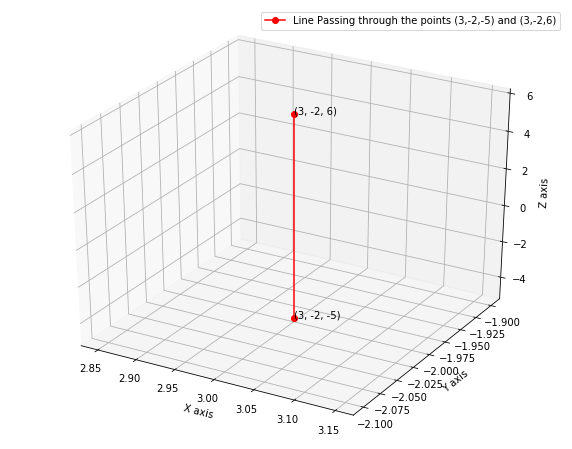
\includegraphics[width=\columnwidth]{./solutions/line_plane/72/assign2.png}
    \caption{Line passing through the points (3,-2,-5) and (3,-2,6)}
    \label{Fig:solutions/line_plane/72/1}
\end{figure}

